\chapter{Analysis}\label{chap:analysis}
\section{What is music? Audiation} 
\begin{quote}
	
	\textit{"Sound itself is not music. Sound becomes music through audiation, when, as with language, you translate sounds in your mind and give them meaning\cite{audiation}."}\\
\end{quote}

Everyone has a meaning about the sound they hear, and the meaning differs from individual to individual\cite{audiation}. Audiation is the concept of assimilating and comprehending music heard by the individual, either in the present or in the past. We can also audiate through reading notations, composing contemporary music or improvising on an instrument.
The concept of audiation is similar to the concept of language\cite{audiation}: \\

\begin{quote}
	\textit{"Consider language, speech and thought. Language is the result of the need to communicate. Speech is the way we communicate. Thought is what we communicate. Music, performance and audiation have parallel meanings. Music is the subject of communication. Performance is the vehicle for communication. Audiation is what is communicated\cite{audiation}."}\\
\end{quote}

An individual can begin audiating shortly after hearing music, to give meaning to the sound. What the individual can take from the audiation depends on that particular individuals previous audiations\cite{audiation}. The concept is similar to regular conversation; if a group of people are talking, each individual will take their own comprehension of the conversation with them. This comprehension is based on existing knowledge and experience of the topic\cite{audiation}. 
The concept of audiation increases the chance of remembering what the individual learns in the long term. Everyone can remember 7 $\pm$ 2 things\cite{gestalt}, however, if the individual tries to remember something without comprehending it, it can easily be forgotten. If students have issues with vocal or instrumental techniques, or they struggle with memory issues, it is most likely due to them not auditing while playing or singing. If the student audiates away from their instrument, technical and memory issues, can be corrected. Instruments should not be seen as the tool to learn how to understand music, but rather the tool to express the music\cite{audiation}.\\

Audiation potential itself cannot be taught but rather depends on how natural, musical aptitude comes to the individual. However, while audition potential cannot be taught, students can be taught how to maximize their musical achievement\cite{audiation}.\\

The technical and memory issues become evident if the students do not learn audiation, notation and music theory in the proper sequence, they will be unable to make sense and add meaning to the sound and music they hear or the notations they read. If the students are unable to tonally audiate what they see in the notations, but still manipulate the keys or valves on the instrument as the notation instructs, the student will often fall out of tune.
Everyone can learn some degree of music. Similar to how everyone has at least some amount of intelligence, everyone has some amount of musical aptitude, so put in other words, everyone is musical\cite{audiation}. Everyone is capable of learning to listen to, and perform music to some extent of success\cite{audiation}. Generally, two-thirds of humans are average, that includes average music aptitude\cite{audiation}.\\

The foundation, that is created in the early years, is a substantial influence on the musical achievement of the student. Most likely, the guidance received in the early stages of their musical careers is a bigger influence, than the guidance the students receive at colleges and universities\cite{audiation}. If the student's musical skill set is not properly maintained, it will severely decrease over time\cite{audiation}.
In order to maintain the skill set properly, the techniques used by teachers have to be considered, as they are highly important\cite{audiation}. When it comes to tonation, the rhythm patterns and harmonic patterns are the most prevalent techniques, and they have remained similar for a long time across different nationalities and cultures as they belong to the basics of audiation. On the other hand, there are activities that include larger classrooms. These will vary a lot depending on the culture, age, and experience\cite{audiation}.\\


\section{Why learn music? The impact of musical education}
Learning audiation and music in general, is not only good for a musical career; several studies have shown that different types of musical engagement in a variety of ways, over a lifespan has an impact on personal growth and development. As concluded in the article \textit{"The power of music: Its impact on the intellectual, social and personal development of children and young people"}:\\

\begin{quote}
	\textit{"This overview provides a strong case for the benefits of active engagement with music throughout the lifespan\cite{powerOfMusic}."}\label{quote:powerOfMusic}\\
\end{quote}

Linguistic abilities and musical training seems to be linked, due to shared brain mechanisms being used to process music and language. Precision in the perception of speech related contrasts, in pitch patterns and other distinctive speech elements have been reported to be associated with musical ability\cite{languageSkills}.\\

A study focused on literary skills showed that a group of second grade students(n = 47) taking piano lessons over a 3-year period had significantly better vocabulary and verbal abilities than a group of control students(n = 57) that did not receive music lessons\cite{vocabularySkills}.
Some aspects of mathematical skills have also been proven to be improved by musical training. For example the subdivision process required to read and play from music scores in order to play and keep a rhythm\cite{powerOfMusic}.
Other abilities have also been reported to be affected by musical training such as creativity, social and personal development, physical development, health and well-being\cite{powerOfMusic}.\\

According to the article \textit{Interactive music video games and children's musical development} there are 5 basic music elements that should be learned in order to get a good understanding and appreciation of music\cite[p.~99]{interactiveMusicVideoGames}:
\begin{itemize}\label{list:basicMusic}
	\item Duration
	\item Pitch
	\item Tone color
	\item Dynamics
	\item Structure\\
\end{itemize}

In another study, which focused on the integration of music in the elementary classroom, results were positive\cite{musicIntegration}. Musical activities activate both the analytical and creative side of the brain, and learning about other subjects becomes easier with the addition of a musical element, as the speed at which information is processed increases\cite{musicIntegration}. An example of this, is learning the math of money exchange through music note denotations\cite{musicIntegration}.\\

\section{Initial problem statement}
Through the initial research, it can be assumed that musical education is important for the development of young students in many facets of life. However, more research is needed to establish what specific aspects of the education can be improved. Therefore, the initial problem statement of this report is as follows:\\ 

\textit{How can a tool improve musical learning in an Elementary school?}

\section{Learning}

In order to establish how music is learned, some research on learning in general was conducted. This chapter will focus on how learning occurs, with a focus on how passive and active learning each have their advantages and disadvantages.

\subsection{Learning Defined}\label{sec:learning}
Learning is the process described as obtaining or modifying knowledge\cite{wikiLearn}. The ability to learn exists for most living things i.e humans, animals, plants and some machines\cite{wikiLearn}. \\

There are many types of learning, this section will mainly focus on Active Learning and Passive Learning due to them being the main types of learning, when talking about education\cite{wikiLearn}.

\subsection*{Passive and Active Learning}\label{sec:activeLearning}
Passive and Active learning are two different approaches and levels of including the student in the material to be learned. 
Passive learning is teacher-based, where the students are not directly involved\cite{activelearning}. This form of teaching is usually seen on universities where the professors gives a lecture, and does not provide assignments or feedback to the students. The approach works on a receiving level, meaning that the student, will learn by hearing and seeing\cite{activelearning}.  
Active learning on the other hand, comes from a person taking control of their own learning experience, and is when the student actively does more than listen\cite{activelearning}. They read, write, discuss, and engages themselves in the given topic. This also includes doing exercises and solving topic specific problems\cite{activelearning}. This approach reaches a \textit{"participating and doing"} level of working with the material. 

Active and passive learning relates to the retention of learning.
The retention of learning is the concept describing the processed information moving from the short term memory to the long term memory\cite{retention}. Furthermore, retention of learning describes how processed information can be forgotten. Attending a lecture without actively participating except listening, can cause a person to lose the up to 70\% of information obtained, within 24 hours\cite{retention}. Multiple theories within the retention of learning also suggests that the information is not lost, but a person is just unable to recall the information \cite{retention}.
In \autoref{fig:activelearn} the concept behind retention of learning is displayed. The figure displays how different ways of learning affects the amount of information learned and remembered. In the bottom bracket, there is the lectures, reading and audiovisual elements. These are the elements which do not actively include the student when obtaining the information. This is the least effective way of learning\cite{activelearning}. In the middle bracket, demonstration, discussion, exercises, and play is displayed, these elements provides a hands-on approach to learning and increases the amount of information obtained significantly\cite{activelearning}. This means interaction and taking an active part in solving a problem, will increase the chance of remembering information about the topic. It is in this and the top bracket, that we find active learning. In the top bracket, there is the "learning by doing" aspect, which contains working with a coach and practice. These last aspects are likely to provide the best results\cite{activelearning}. This is because there is a personal approach and the motivation by the student is higher at this point\cite{retention}. 

\begin{figure}[H]
	\centering
	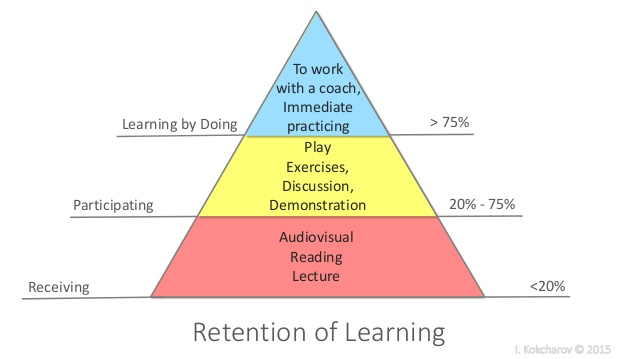
\includegraphics[width=0.9\linewidth]{figure/Analysis/skillslearn}
	\caption{Retention of Learning from Kokcharov's Skillpyramid\cite{skillPyramid}}
	\label{fig:activelearn}
\end{figure}
\todo{Instead of "here" in the caption, we need to add a name, author, webpage or something}
\todo{Also, write caption that describes figure, don't do this in the above text.}

\subsection*{Sub Conclusion}
In an educational environment, both active learning and passive learning are being utilized. Based on the findings, active learning will provide a better learning experience where the student will be able to remember more information. This means that participation and practice optimizes the learning experience the most.\\

\subsection{Interaction in a learning perspective}\label{sec:interaction} 
As mentioned in \autoref{sec:learning} a hands-on approach and interaction is important to get an efficient learning experience. This chapter will focus on and go in depth with interaction in correlation to learning.\\

Interaction is described as when objects or people interact with each other, this can be a person interacting with an object, or an object interacting with another object etc.\\

As mentioned in \autoref{sec:learning}, it is important that the students and the teachers are actively involved in the learning activities, to achieve as much as possible from their learning experience. Students should have an opportunity to interact with teachers as well as the other students, to increase their learning opportunities. The teacher should provide a classroom with room for involvement and motivation in the learning process\cite{interactionlearning}.\\

A different view of interaction in a learning perspective, is not only the interaction between students and teachers, but also a hands-on approach for the students when learning about new subjects. This is also referred to as kinesthetic learning or tactile learning\cite{kinest}. Kinesthetic learning is what describes a student carrying out physical activities rather than listening passively to a lecture\cite{kinest}. This learning by doing approach is among the most popular learning methods among the students\cite{kinest}. This method gives the students space to learn from their mistakes\cite{kinest}. \\

Many people will learn more with kinesthetic learning, where movement using more senses will improve their learning outcome and learning experience\cite{kinest}. In the book \textit{The Kinesthetic Classroom: Teaching and Learning Through Movement}\cite{kinestheticMovement}, it is argued that movement induces cognition, an argument that is supported by Dr. John Ratey\cite{rateySpark}. Ratey argues that exercise before having classes improves focus and mood for students\cite[p.~33]{rateySpark}. This relates to active learning seen in \autoref{sec:activeLearning}, and kinesthetic learning in \autoref{sec:interaction}, as both relate to either being active or being physical doing learning.

\subsection*{Sub Conclusion}
To improve the learning experience and the learning outcome, it is important to incorporate interaction in the studies. Giving the students the opportunity to interact with a topic which they are learning about, will increase their chance of remembering information and give them an easier time to learn it. Interaction can extend to incorporating more movement and is not excluded to hands-on approaches.

\subsection{Motivation}
Motivation is an integral part to learning, and is therefore important when looking at ways to assist children in learning music\cite{motivationGameDesign}. The most fundamental motivational theory is the one called Self Determination Theory (SDT)\cite{SDT}. SDT proposes that motivation is divided into two brackets; Intrinsic motivation and extrinsic motivation\cite{SDT}. 

\subsubsection*{Intrinsic motivation}\label{sec:intrinsic}
Intrinsic motivation is the internal motivation, that pushes humans to do actions not depending on a specific reward, but wholly depending on the inner need to do the action, for the sake of it.
This is the inherent need humans have to learn, explore and widen their knowledge\cite{SDT}.\\

To establish what influences intrinsic motivation, the researchers behind SDT created the Cognitive Evaluation Theory(CET) as a sub-theory within the existing SDT\cite{SDT}. CET is the theory that focuses on competence and autonomy in relation to intrinsic motivation. The first part of the theory says that social-contextual events that contribute to the feeling of competence for a performed action, improve the feeling of intrinsic motivation in relation to that action\cite[p.~70]{SDT}. These social-contextual events might include rewards, feedback and communications\cite[p.~70]{SDT}. For intrinsic motivation to be improved, the action that is performed must be accompanied by a feeling of autonomy\cite[p.~70]{SDT}.

\subsubsection*{Extrinsic motivation}
Extrinsic motivation is the motivation that drives a person, depending on a reward associated with the performed action. From the SDT theory extrinsic motivation is defined as: 
\begin{quote}
	\textit{The term extrinsic motivation refers to the performance of an activity in order to attain some separable outcome.}\cite[p.~71]{SDT}.\\
\end{quote}
An extrinsically motivated action could be; performing a non enjoyable job, meaning that there is no intrinsic motivation to the work, however when a paycheck is included, the action is extrinsically motivated\cite{SDT}.

\subsubsection*{Emotions}
Emotions and motivation have a sort of bidirectional relationship in which each side can activate or deactivate the other\cite[p.~66]{emotionsAndMotivation}. In addition to that, emotions directly impact the quality of learning\cite[p.~66]{emotionsAndMotivation}. In the book \textit{"Emotions and Motivation in Learning and Performance"}\cite{emotionsAndMotivation}, they use an example with a student named Jake, he has had past negative experiences with studying. This deactivated his motivation to study in the future, because the negative emotions relating to the bad experience interrupted his goal of studying\cite[p.~67]{emotionsAndMotivation}. To better counter the negative emotions, and deactivation of motivation, one must consider highlighting the intrinsic task value of an action\cite[p.68]{emotionsAndMotivation}.

\subsubsection*{Sub conclusion}
Whether motivation is extrinsic or intrinsic, it is a core part of performing any action. Thinking about learning, the intrinsic task value should be considered to be highlighted, so as to counter negative emotions, specifically the concept of social-contextual motivation is effective.

\subsection{Collaborative learning}\label{collabLearning}
 Seen through a biological perspective, humans are social animals\cite{laeringIPraksis}. This has a high influence on the process of learning, since humans, as pack animals learn with and from each other, the learning process is social\cite{laeringIPraksis}. Working in groups and teaching each other, therefore strongly appeals to the human brain, and can be considered a powerful impacter when learning\cite{laeringIPraksis}. 

There has been a lot of research on collaborative learning in various educational contexts. However, the more artistic educations have been slightly overlooked\cite{collaborativeLearningTeachers}\cite{collaborativeMusicAnalysis}\cite{collaborativeLearningReview}. 
The article \textit{The Experiences of Elementary Music Teachers in a Collaborative Teacher Study Group} states, based on research outside of a musical context, that:\\
\begin{quote}
	\textit{"collaboration can improve learning outcomes if students make a conscious effort to coordinate their efforts and are able to come to a shared conceptual understanding of the problem being solved"}\cite{collaborativeLearningTeachers}.\\
\end{quote}
However, it is not an entirely unexplored area, studies have shown that musical collaboration stimulates students' critical and creative thinking\cite{collaborativeLearningTeachers}. Rich musical experiences can surface from combining ideas\cite{collaborativeLearningTeachers}. 
The article introduces three principles of collaboration that are based on interviews with three teachers:\\
\begin{enumerate}
	\item Collaboration facilitates student self-expression and independence. This is at work when students, for example, are divided into smaller groups, and find themselves focusing on a task that generates communication, arguments and discussions without the teachers' involvement. They will show independence as they individually will try to convince others to reach the same conclusions\cite{collaborativeLearningTeachers}.
	\item Students who are collaborating share goals. The teacher allows space for, or guides students in creating productive student to student interactions. This is related to a student groups' shared motivation while focusing on a shared goal, for example presenting their work for the entire class, and sharing the responsibility to reach that goal\cite{collaborativeLearningTeachers}.
	\item A teacher collaborating with their students, facilitates their movement toward a shared goal. The teacher provides necessary background skills, creates student incentive for the goal, and then allow students to take ownership. This is a teacher-student collaboration that also can be present within the classroom. Here the teacher will, for example, instruct the student with harmonies, rhythms, chord progressions etc. after which the teacher gradually let the students take control over the task at hand\cite{collaborativeLearningTeachers}.
\end{enumerate}

\subsection*{Sub conclusion}
Collaborative learning lies in the human nature and can be considered a great and positive influence in the learning process. Furthermore, it has an impact on various aspects of personal development such as creativity and social interactions that could be useful later in life.

\newpage \section{Problem Area}\label{sec:problemArea}
In order to establish a target group, the current musical education in elementary schools was analyzed, through a look at the current study plan and an interview with a music teacher at an elementary school. These will help clarify possible improvement within the current musical education.

\subsection{How is music taught? The Study plan}\label{studyPlan}
According to the study plan, found on the website of the Danish Ministry of Education the children are required to learn three areas of competence. These are musical performance, musical creation and musical understanding\cite{studyPlan}.

\subsubsection*{Musical performance}
Musical performance includes teachings about singing, movement, and playing instruments. More specifically teaching the children about how to sing individually and in groups, as well as teaching them about different kinds of singing and songs. Furthermore, it teaches the children about movement in a musical context, such as dancing and rhythmic movement. Finally, it teaches the children to be able to play the basics of different instruments, such as drums, guitar, piano, keyboard, and different wind instruments\cite{studyPlan}.

\subsubsection*{Musical Creation}
Musical creation includes the teachings of different abilities in relation to creation, alternation or improvisation of musical pieces. The children should be able to compose music with the ability to remember time and tempo when creating music. Furthermore, the children should be able to form and shape sound into something rhythmic. Besides creating music, the children should also be able to modify music with the help of adding sounds, or changing the pitch or pace of the sound. Finally, the children should be able to improvise music\cite{studyPlan}.

\subsubsection*{Musical Understanding}
Musical understanding is, to be able to express music in other forms than sound. They should be able to express themselves verbally about music and be able to draw music. The children should have knowledge, about instruments, and the ability to distinguish the different instruments from their appearance, as well as their sound. The children should be able recognize specific elements in a musical piece, and identify them. Finally, they should have the knowledge of musical history, in relation to different musical genres, as well as music from different time periods\cite{studyPlan}.\\

The children will be introduced to digital tools and synthesizers to be used in the classroom. These tools might include iPad or Garageband. On these devices, they are asked to compose a musical piece using the aforementioned knowledge.\\
From the first to fourth grade, the children are working more with analog instruments as well as singing to develop a musical foundation for their education.\\

\subsection{Interview with Hanna Jørgensen} \label{ProblemArea} 
Hanna Jørgensen is a musical teacher at both elementary school level and Danish Gymnasium level at Skt. Annæ Skole. She is also a pedagogue in Musical Pedagogy at the National Music Conservatory. Besides the aforementioned credentials, she is also involved in the “Børne og Ungdoms Forvaltningen”, which is an organization that tries to improve the quality of life among children and young people. She is interviewed to help establish a detailed view on how the current musical education functions, and to help locate issues within the musical curriculum for elementary school children.\\ 

The beginning of the interview focuses on the current structure and tools that Hanna uses in the classroom. Hanna explains that the current study plan, for her class, is divided into courses with focus on a particular musical subjects. According to Hanna, Games and movement are two tools that are important for how music is taught in elementary school. There are currently a set of tools used to teach music through games, but Hanna sees a lack of creative tools that support the education, and there is room for innovative ideas.\\

She also emphasizes the importance of Rhythm. Rhythm is essential for singing, playing instruments, and understanding music. This means that there is a focus is on the learning and understanding of rhythm in elementary schools. Instruments are not used as commonly, as they are harder to get by, and singing provides a tool that everyone possess. When it comes to the theoretical education, Hanna finds it essential to work with visual and physical tools. \\

The collaboration is another theme, that Hanna finds important to teach the kids, however she currently finds a lack of collaborative tools. The class that Hanna teaches uses software such as Garageband, but the interface is limited to a single user at a time. She seeks physical tools that allows for creative thinking when collaborating.\\

\subsection{Workshop}\label{sec:workshop}
The workshop was conducted at Skt. Annæ Skole, which is not a regular public school. It does follow the general study plan of elementary school education, but it has a focus on musical education. Skt. Annæ Skole teaches musical concepts and performance on a higher level than a regular elementary school.\\

The goal of the workshop was to get an idea of what the children thought about their current music education, what tools they use and how these tools could be improved. The children were presented with different ideas for new and alternative tools that can be used in the education. The children were presented with six unique ideas, each based on an initial brainstorm. The ideas were drafted on the basis on the knowledge gathered in the early analysis, and were based on tools the children already used. The children had to provide feedback on the ideas and compare them to existing ideas, to find what elements of the different tools the students desire.\\

Across the different ideas in the workshop, a number of trends became apparent. The following points were the most prominent when it came to desired features:\\


\begin{itemize}
	\item[-] \textbf{Movement}\\
	The children found the current education to be very inactive. They desired ways to be more active and have more movement as part of the education.\\
	\item[-] \textbf{Variation:}\\
	The children disliked using the same tools and same methods for learning various aspects. Having variation to keep things fresh would be more fun.\\
	\item[-] \textbf{Games:}\\
	The children love to learn through games. They feel like they remember a lot of what they learn, when they use games and they have fun while learning. \\
	\item[-] \textbf{Visuality:}\\
	The children asked for more visual components in their education. It is important to them that what they use are presented in front of them visually and had colors that were pleasing to look at.\\
	\item[-] \textbf{Physical:}\\
	The children loves when the tools are physical. If they can see, touch and feel the objects they use to learn, they have more fun and feel like they learn.\\
	\item[-] \textbf{Group work:}\\
	The children expressed great joy about working together with their classmates and collaborating in different ways about creating and understanding music.\\
	
\end{itemize}



\subsection{Target Group} \label{sec:targetgroup} 
Based on an analysis of how the current education is, and how the students perceive it, the target group for this project are children aged 8-12, currently attending a musical education in elementary school.\\

The music teachers will be considered a sub target group, as the tool would have to be used and explained by the teacher. The teacher would have to use the tool to provide knowledge and add meaning to what the tool represents.
 
\subsection{Learning tools used}%Mini SOTA
This section is about the learning tools that Hanna Jørgensen mentioned in the interview in \autoref{ProblemArea}.  

\subsubsection{GarageBand}
GarageBand is a software developed by Apple Inc, as seen in \autoref{fig:garageband}. It is used for allowing users to create, edit, and render music. The whole idea of GarageBand is that the software uses pre made MIDI keyboards, loops and arrays of different instrumental effects and voice recordings that can help the user further develop various sounds. This software is a very helpful tool for learning how to create music.
\begin{figure}[H]
	\centering
	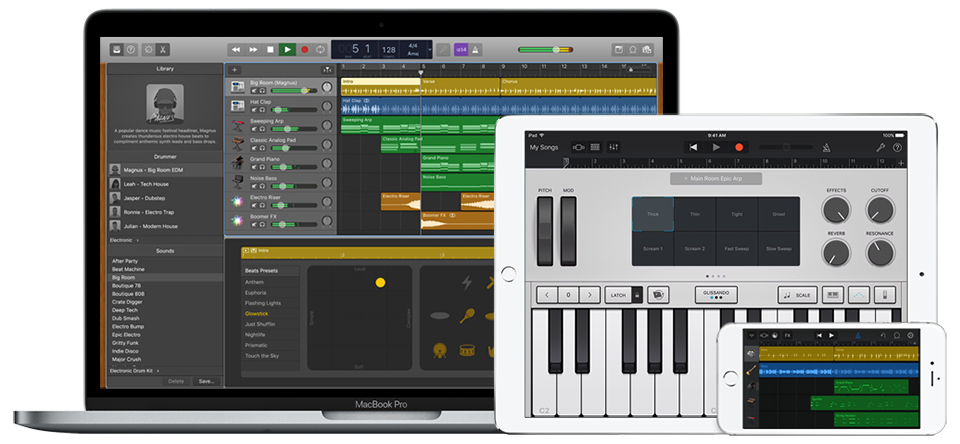
\includegraphics[width=0.7\linewidth]{figure/Analysis/garageband}
	
	\caption{Shows the GarageBand's interface}
	\label{fig:garageband}
\end{figure}


\subsubsection{MuseScore}
MuseScore (seen \autoref{fig:MuseScore}) is an open-source software program for creating music notation. The main attraction of the software is the ability to play and practise sheet music anywhere. You are able to search for new music sheets and practice these by either listening to the notes or change the notation. It is available for windows, mac, IOS, Android, and Kindle Fire. It accepts an input via MIDI keyboard and can transfer to and from other programs via MusicXML, MIDI or others. This is a very useful tool for understanding and practise music notation. The program is build so that anyone is able to create music.

\begin{figure}[H]
	\centering
	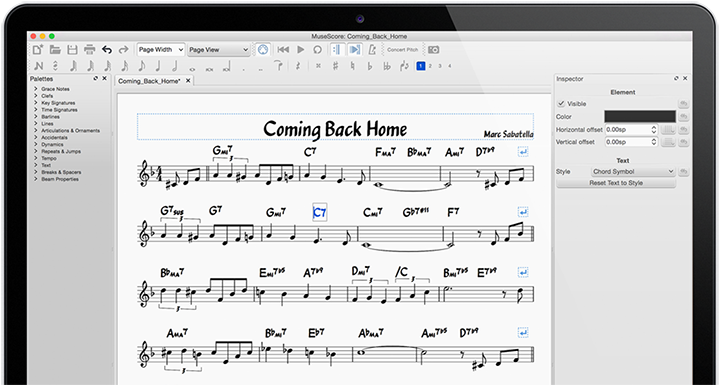
\includegraphics[width=0.8\linewidth]{figure/Analysis/musescore.png}
	\caption{Shows a picture of sheet music that can be played or manipulated, to understand the music notation}
	\label{fig:MuseScore}
\end{figure}

\subsubsection{Go Fish - Music notation} 
Go fish is a card game played by two or more players. The rules state that five to seven cards are given from a standard 52-card deck to each player. The remaining cards are spread out on a table. When it is a players turn, that player can ask any other players if they have a card of a given value. If they do, that card is given to the player that asked and if they don’t the player is asked to “go fish” which means the player who asked, has to pick a card from the pile of cards on the table. To win is to gather as many sets of cards of the same value. Hanna from Skt. Annæ is playing this game with her students where she do not use the standard 52-card deck, but uses cards with music notation; Making it a learning tool for people to memorize or learning the different notations of music. Seen in \autoref{fig:gofish} is an example of go fish looks with notes.

\begin{figure}[H]
	\centering
	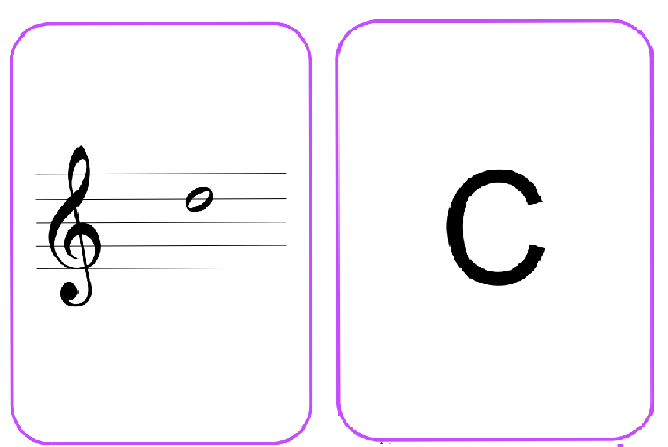
\includegraphics[width=0.7\linewidth]{figure/Analysis/gofish}
	\caption{An example that shows how Go fish can be played with notes}
	\label{fig:gofish}
\end{figure}

\subsubsection{Sibelius}
Sibelius is a software program for creating music notation. It was created by Sibelius Software. The software can edit, print, play the music using synthesized sounds, and produce scores. It can be used for playing the music or turning it into audio files. It supports basically any MIDI device and it also comes with some pre made sample files. In \autoref{fig:sibelius} a picture of what Sibelius looks like, can be seen. 

\begin{figure}[H]
	\centering
	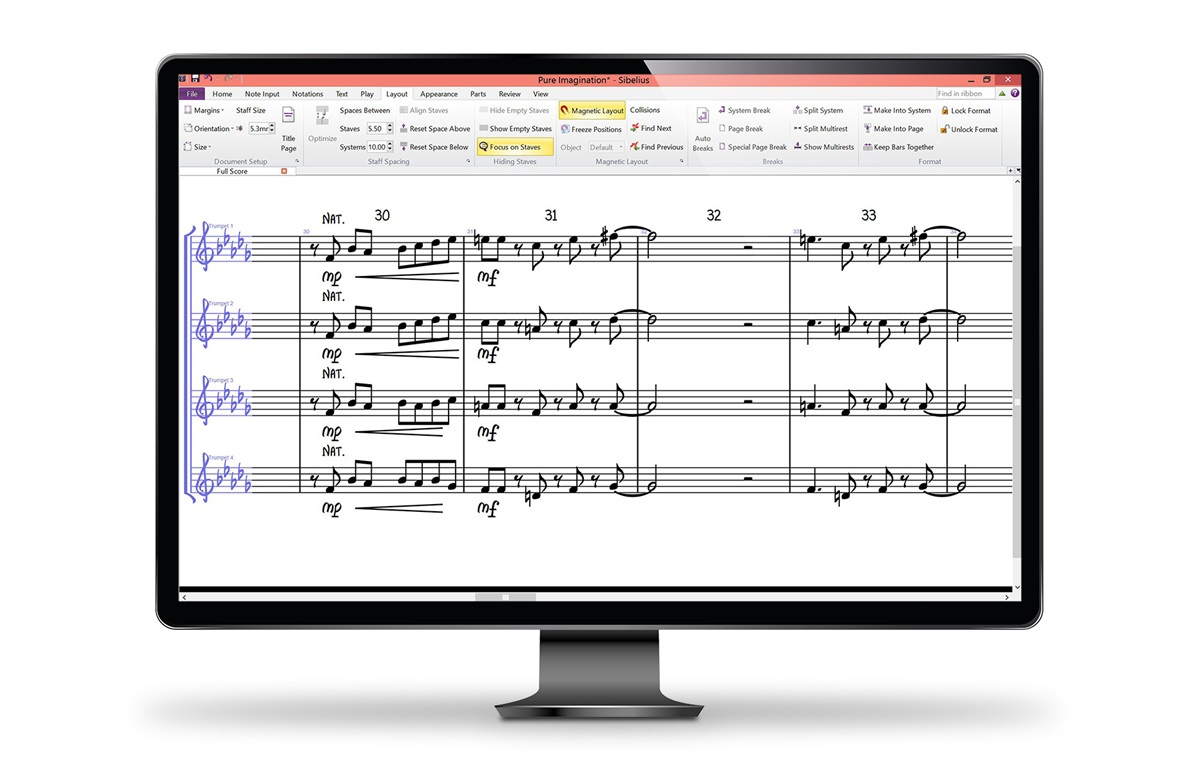
\includegraphics[width=0.7\linewidth]{figure/Analysis/Sibelius}
	\caption{Shows what the software looks like with different notations}
	\label{fig:sibelius}
\end{figure}

\subsubsection{Clio Online} 
Clio Online is an online tool for students who wants to learn more about the different topics. You can learn topics such as Danish, English, German, religion, history, biology, sports, music, arts, food etc. This is a tool used by teachers to help their students with their studies. In every subject there are help tools such as videos, sound files and pictures to optimize each users' learning pattern. This online tool also provides the user the capability to choose what difficult level the material should be.

\subsubsection{Music work out}
Music work out is a physical tool-set developed by Anette Præst Nielsen, as seen in \autoref{fig:musicworkout}. It is a box consisting of different games or teaching methods for users who want to learn or have fun with music. There are currently two different editions; a teacher’s edition and a Game edition. The teacher’s edition contains around 800 cards and accessories. It is used for learning about music theory, notes- and ear training, rhythm cards, interval cards, rest cards, time signature cards, solmization cards, subdivision cards, clef card etc. The game edition contains 3 different games; Domino, Bingo, and Memory. Which also consist of different parts of the above topics.

\begin{figure}[H]
	\centering
	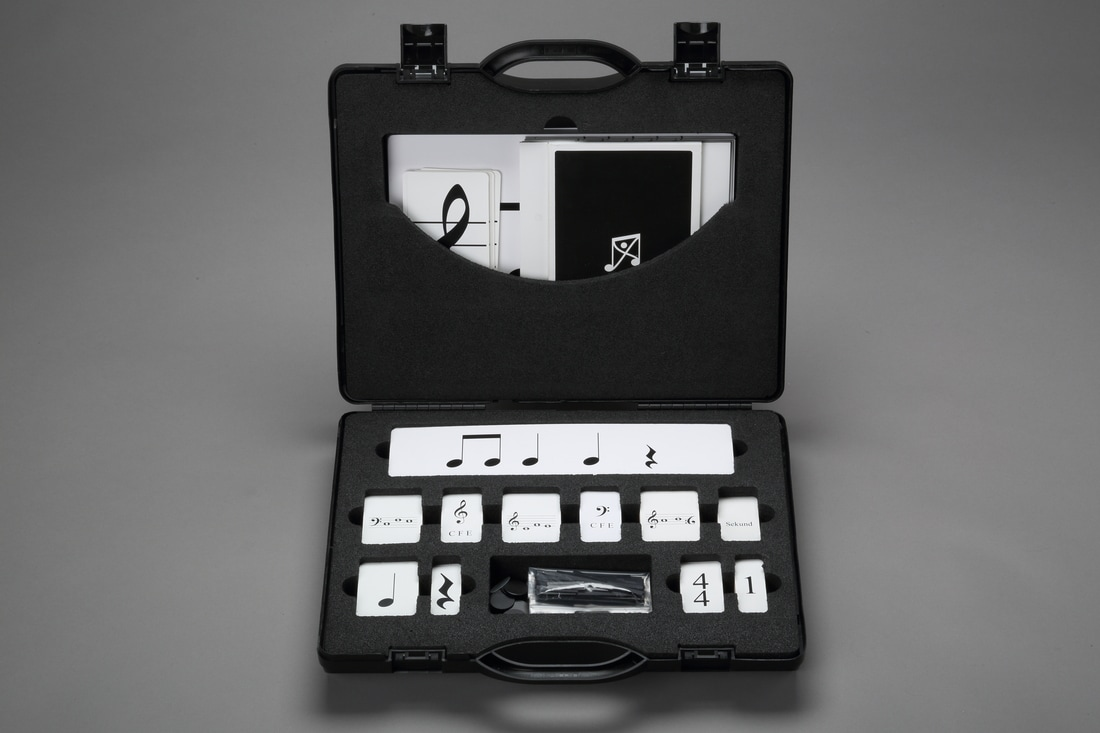
\includegraphics[width=0.7\linewidth]{figure/Analysis/musicworkout}
	\caption{An example of the teacher's edition for learning about music notation}
	\label{fig:musicworkout}
\end{figure}

\subsection{Choice of Direction}
The knowledge gained in the problem area chapter, provides a direction for the progress of the project. A look at the study plan gives an overview of how the schools currently teach music throughout the three areas of competence; Musical Creation, Musical Understanding and Musical Performance. An interview with Hanna Jørgensen provided insight into current issues with the musical education, which leads to an analysis of the potential target group.\\

With the target group established, an analysis of the tools currently being used by the target group, in the context of the information gathered throughout the interview and a workshop. This highlighted issues with a lack of physical tools, that the target group can use to learn music in collaboration with each other. The children in the workshop expressed issues with the lack of tools, that can be used when working in groups.\\

The following analysis will focus on the aspects found in the problem area. Collaboration and how working in groups affect learning will be researched.\\

\section{Working in groups - different aspects and approaches} % Sofie (sammenflet)
When working in groups, different aspects affect the productivity and level of performance and thereby affects the learning outcome for both the group and individuals\cite{GodKlassekultur}. In this section some of these aspects will be discussed. These include: The arrangement of groups, the teachers role, roles within a group, inclusion and exclusion from a group, feedback as an important group tool, and different collaborative learning methods such as cooperative Learning, constructive competition, and peer Learning.

\subsection{Group sizes}\label{GroupArrangement}
The number and sizes of the groups need to be taken into account, and correspond to the total number of students and teachers within the class. Assuming that there is a classroom with 32 students a grouping of 4 students in each group will mean that a teacher needs to prepare and manage 8 groups which can be more difficult. Fewer larger groups with more members, 6-8 students, however, will be more convenient for a teacher to manage, but the learning outcome of the individual students within the group might not be ideal\cite{collaborationSocialPedagogy}. The smaller the groups the better the cooperation and beneficial effects of competition can arise\cite{collaborationCompetitionGames}.

\subsection{The roles within a group}
Group stability and dynamics are other factors that teachers might need to consider. It might be more beneficial for the students to be arranged in groups based on the teachers prior knowledge about the students' behavior and stick to the same groups for longer periods\cite{collaborationSocialPedagogy}. This gives the group time to challenge the knowledge of the group, and learn the members differences and thereby gain understanding of the importance of different work approaches and processes\cite{laeringIPraksis}.

Differences among people when working in groups are important, as the group members contributes in different areas (academically and socially), and can thereby overlap each others strengths and weaknesses\cite{ProjektarbejdesKompleksitet}. These individual collaborative roles, inspired by Belbins' team roles\cite{ProjektarbejdesKompleksitet} can be categorized in three main categories: 
\begin{itemize}
	\item[-] The thinking role - focus is being creative, making ideas, and the outcome of the work. 
	\item[-] The doing role - focus is the process of the work (how and why).
	\item[-] The social role - focus is the well-being of the group. 
\end{itemize}

Having a representative from each category strengthens the group work and the result, and thereby the learning outcome\cite{ProjektarbejdesKompleksitet}. However, if not represented and the importance of each role is not acknowledged, it can lead to conflicts within the group. These conflicts, can often be seen as difficulties within certain areas i.e. problems with organizing, leading to unstructured work, or the feeling and expression of a not equal contribution, which can lead to social conflicts \cite{ProjektarbejdesKompleksitet}. 

\subsection{Social inclusion and exclusion}
Being a part of a group lies within human nature and is important for the individuals well-being as well as their motivation, and can therefore effect the learning process\cite{ProjektarbejdesKompleksitet}. Being excluded from a group has a negative effect on the individuals learning and social well-being. This can even influence the person being excluded to avoid future group work due to the psychological defeat. The Danish professor in social psychology Dorte Marie Søndergaard, calls this \textit{social exclusion anxiety}\cite{ProjektarbejdesKompleksitet}. Being excluded is often related to the contributions' value. If the group members' contribution does not meet the requirements or is seen as of less value, exclusion can occur. Exclusion can also be caused by character traits and personality, and might therefore not necessarily originate from academical skills\cite{ProjektarbejdesKompleksitet}.
To reduce the risk of exclusion and facilitate inclusion, the group must function socially and understand the importance of the different collaborative roles. The tasks that groups need to complete have to be designed in such a way that they encourage collaboration and discussion, and does not promote individual work, in order to produce an effective learning outcome\cite{collaborationSocialPedagogy}. To further enhance inclusion, feedback can be used. 


\subsection{Feedback}
Feedback given between members of the group, is a highly important part of group work\cite{laeringIPraksis}\cite{ProjektarbejdesKompleksitet}. It is with this tool that the group can reflect on their work, and together work towards a shared goal, improving the learning process and outcome for both group and individuals\cite{laeringIPraksis}\cite{ProjektarbejdesKompleksitet}. It is also a tool which can be used to acknowledge each others work, and enhance inclusion and social well-being\cite{laeringIPraksis}\cite{ProjektarbejdesKompleksitet}. 


\subsection{Collaborative learning Methods} 
When collaborating, the process and methods must relate to the type of work. Collaboration can therefore be conducted in many ways. In the following sections three acknowledged collaborative methods, namely \textit{Cooperative Learning, Constructive Competition, and Peer Learning}, will be discussed.  

\subsubsection{Cooperative learning}
A term which is used widely within the category collaborative learning(see \autoref{collabLearning}), is cooperation\cite{collaborationCooperation}. It is a teaching strategy in which children in smaller groups in a class room cooperate towards a common goal and thereby develop their social skills whilst building a common base of knowledge about a course subject\cite{collaborativeLearningTeachers}\cite[p.~15]{peerLearning}\cite{collaborationCompetition}\cite{cooperativeLearningPractice}. A teacher divides the children into smaller groups for either a long or short term period and assigns a task to them. The children are thereby responsible for each others learning, and cooperate towards the groups' success in solving the task. Meanwhile, the teacher walks around between groups and monitors their progress\cite{cooperativeLearningPractice}. Even though cooperative learning has shown positive results in learning outcomes of the children, it has also been criticized.In some cases, the children will be taking on a larger part of the work, while others do nothing. Cooperative learning has also criticized for the risk of causing competition between either group members or whole groups\cite{collaborationCooperation}.

\subsubsection{Constructive Competition}
Competition tends to be seen as a negative and destructive force when talked about in a learning context and is often conceptualized as an opposite to collaboration\cite{collaborationCompetition}. Humans compete to outperform others in various situations such as at work, in school or in games\cite{collaborationCompetitionGames}\cite{collaborationCompetition}. However, in the right conditions, it can be constructive as it is simultaneously a strong motivator in learning situations\cite{collaborationCompetitionGames} and makes children perform beyond their own expected abilities\cite{collaborationCompetition}. Competition is one of the core mechanics in video games and aside from  motivation, it increases excitement, involvement, attention, and if such a game is educational, these effects could potentially have positive effects on learning\cite{collaborationCompetitionGames}. 

\subsubsection{Peer Learning} %Sofie
In peer learning, equal individuals work together in peers to achieve their individual goals\cite{peerLearning}, often in a tutor-mentor or tutee-mentee relationship. The idea is, that through mutual help and support, knowledge should be shared between them, the goals will then be to either learn by teaching or by being taught. This can be done in different constellations\cite{collaborationCompetition}.

\begin{description}
	\item[Peer Instruction] The children arrive prepared to given course, the teacher asks a question about the subject, and the individuals state their answers. Next, the assigned peers discuss the question and based on this, state their reevaluated answers. In this process the students have prepared themselves about the same material, and so their knowledge might not vary significantly, and the roles of tutor and tutee might not be present.\\
	
	\item[Peer Tutoring] Each of the peers must prepare and be able to teach a given material, to another peer. The peers is therefore in the roles of \textit{tutor} and \textit{tutee}, and shifts roles after a certain amount of time. This process relies on the fact that each of the peers have a greater understanding of different subject than others, as the roles of tutor and tutee will become present.\\
	
	\item[Peer Mentoring] This resembles the process of peer Tutoring, but instead the students must have different skill and experience levels i.e. comes from two different grades. Instead of a tutor and tutee, the terms \textit{mentor} and \textit{mentee} is often used, as the social relationship is often more in focus, than achieving academically skills.\\
\end{description}   

For all different approaches to peer learning, it applies that the teacher must have a deep understanding of the individual students, both in terms of social and professional skills \cite{collaborationCompetition}. Otherwise the Peers might not have the right prerequisites for the collaboration\cite{collaborationCompetition}.


\subsection{Sub conclusion} %Sofie og Jens
Understanding how the teacher should form groups, and how the dynamics of the group affects the work, will help in understanding how a design strive to relate and support both these arrangements and collaborative roles. Inclusion will provide a higher learning outcome for both the group and for the individual. The collaborative methods can act as guidelines for the design and usage of the tool.\\

As most of the factors concerning group forming, dynamics, and arrangements,  will be in the hands of the teachers, they might not be something that can be directly designed for.  
However, based on the section's findings, the tool ideally could be used for groups of the size 2-6 students.
 
\section{State of the art - Design Inspiration}\label{sec:sota}
In this part of State of the art, the focus was on analyzing design inspiration. It provided insight into physical and digital interfaces. Each design inspiration uses at least one of the three learning methods; cooperative learning, constructive competition and peer learning, but will only state some of the connections each learning method provides.

\subsection{Guitar hero}\label{sec:guitarHero} 
Guitar Hero is a game developed for playing music with components that resembles instruments. The idea is that the player will see notes on the screen in different colors, seen in \autoref{fig:guitarHero}. Each color is represented on a controller that is shaped like a guitar.  The player then have to match and press the correct color on the controller, at the right time. Guitar Hero makes use of some aspects of constructive competition, due to having a point system where the better player would have more points. In addition, it also uses aspects from cooperative learning, by having shared health system where when played incorrectly, health will decrease and if it is depleted, all players lose.
 
\begin{figure}[H]
	\centering
	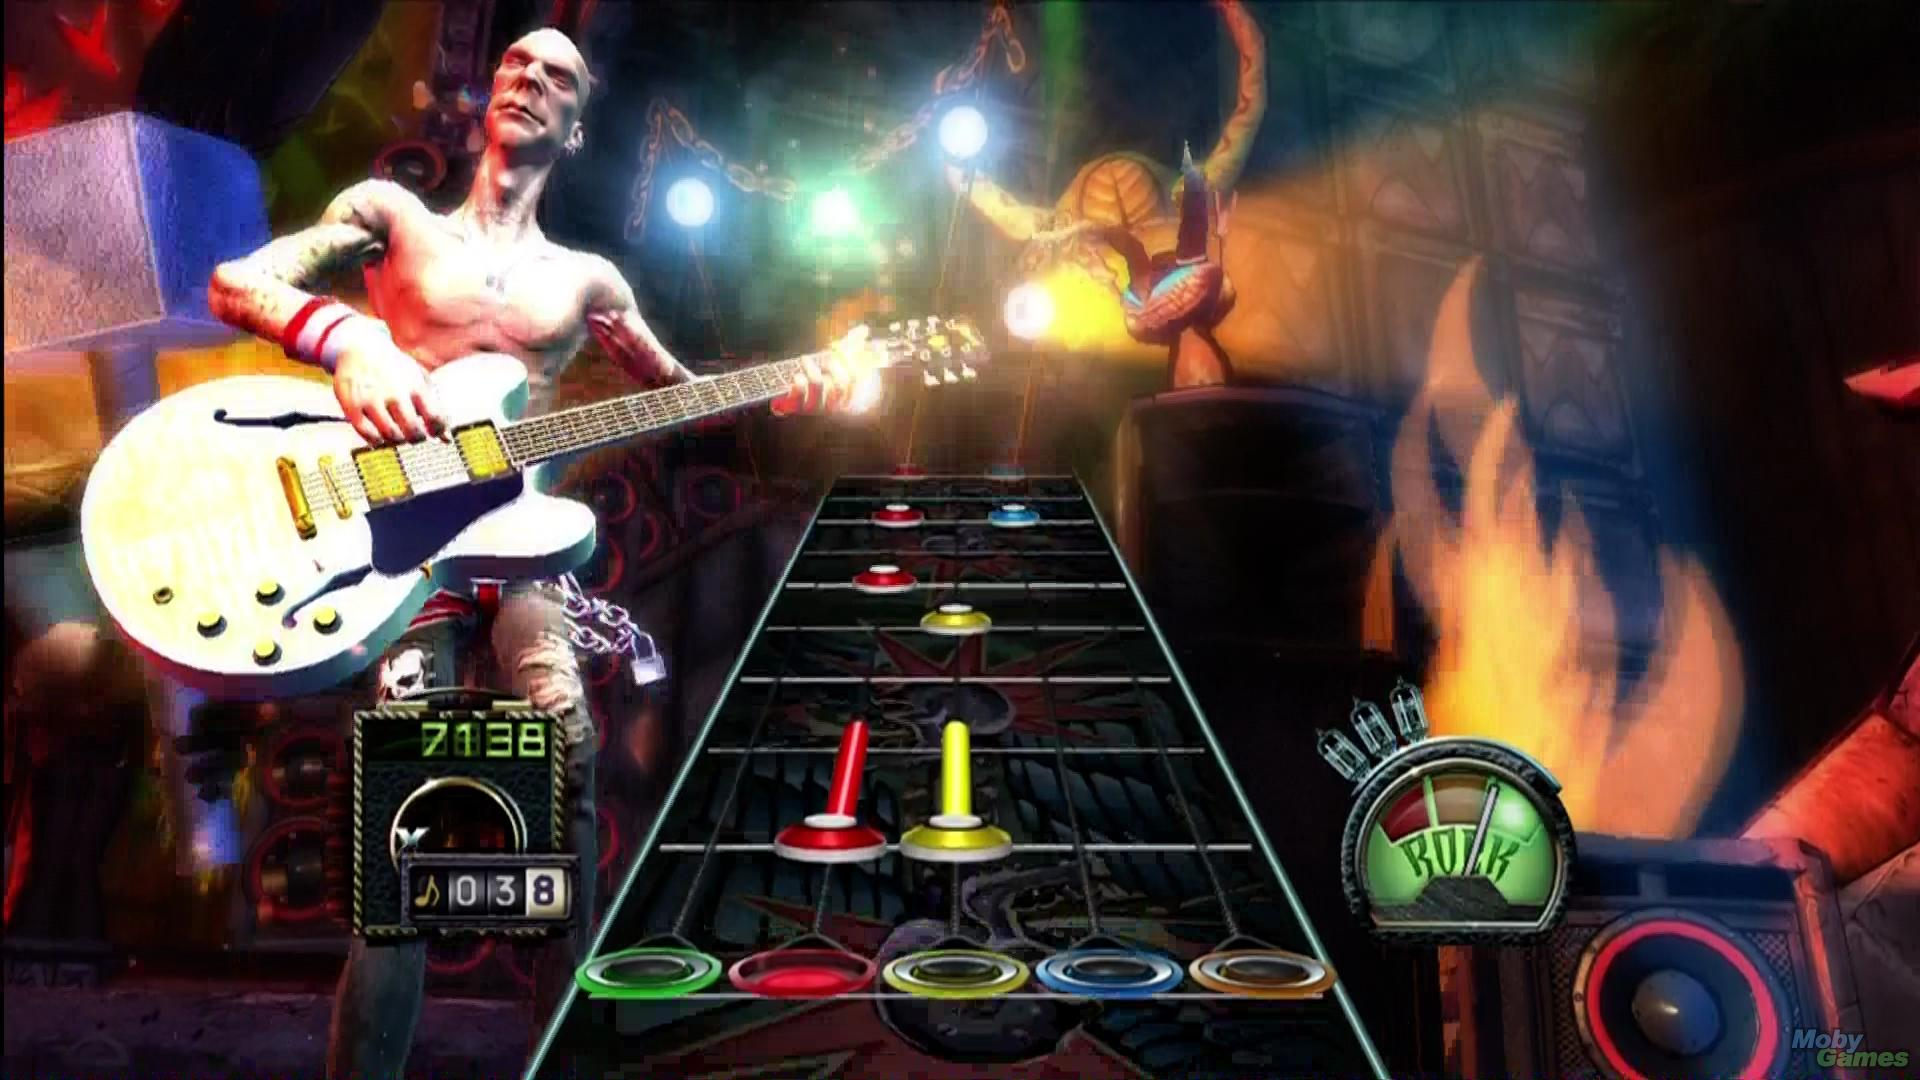
\includegraphics[width=0.7\linewidth]{figure/Analysis/guitarhero}
	\caption{The Guitar Hero interface}
	\label{fig:guitarHero}
\end{figure}

\subsection{Noteput} 
Noteput is an interactive music table with tangible notes, for learning notation. The idea is that you use the interactive screen that shows a staff which can be either a Treble Clef or Bass Clef. You can choose between the different notations and place them on the staff, to determine if they should be whole, half, quarter, eights, sharp, flat or natural notes, as seen in figure \autoref{fig:noteput}. The table also has an option to play or loop the sounds, so that the user can keep changing the sounds as the loop keeps playing. 

During the workshop is was established that the children wanted more movement, variation, gamification, visuality, and physicality which makes Noteput an inspiration for further development. The important parts of Noteput is the physical and tactile interface.

\begin{figure}[H]
	\centering
	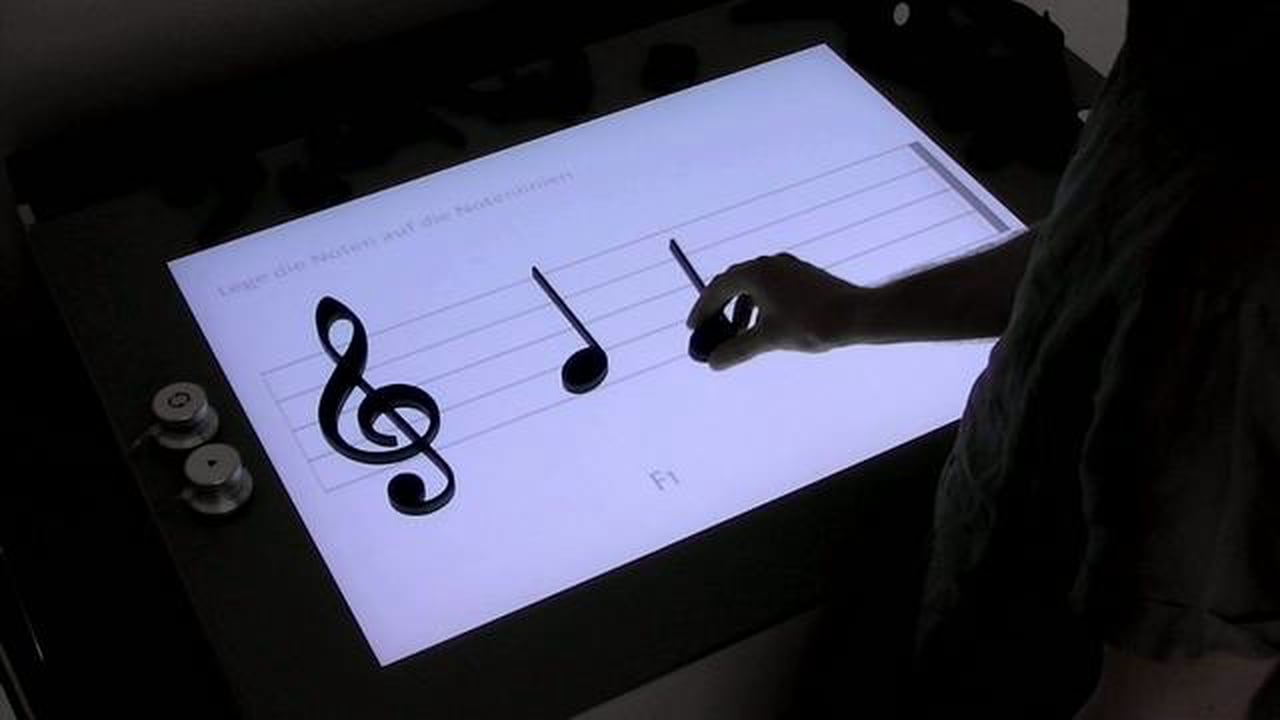
\includegraphics[width=0.7\linewidth]{figure/Analysis/noteput}
	\caption{Shows a user placing tangible notes on the interactive screen}
	\label{fig:noteput}
\end{figure}

\subsection{Dato Duo} 
Dato Duo is a two person synthesizer. Dato duo is a combination of a synthesizer and sequencer for creating electronic music together. It can be played alone or with others. On one side it is build using the circular sequencer which loops the last eight notes that is played. On the other side are the controls for the synthesizer, which contains two sliders that controls the two digital oscillators and the filter-cutoff frequency. It can also be combined with MIDI components. Dato duo can be used for cooperative learning because the users will be making music together and helping each other in their task, as seen in \autoref{fig:datoduo}.

It can be played alone but is best used together with other people. The device focuses on giving each user different components to control. Each component helps the users combine sounds, and make the device more collaborative when making sounds together.
\begin{figure}[H]
	\centering
	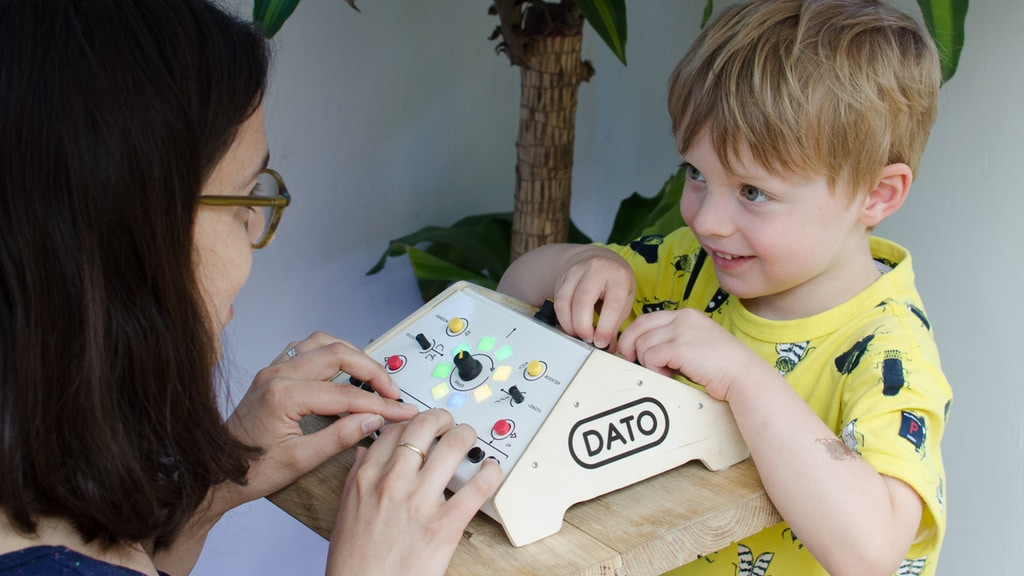
\includegraphics[width=0.7\linewidth]{figure/Analysis/datoduo}
	\caption{Shows the Dato duo synthesizer being interacted with by two users}
	\label{fig:datoduo}
\end{figure}

\subsection{DropMix}
DropMix is a hardware instrument for music creation or mixing, and can be seen in \autoref{fig:dropmix}. It uses a large board with five different slots for placing cards with different values. It is operated by using a phone or tablet. There are three different modes, which are clash, party, and freestyle. Clash mode is a competitive game for two to four players. The goal of Clash is to be the first team to reach 21 points. Each card that is placed on the table scores a point. To replace a card in one of the slots, it must be either equal or a higher value than the card already in the slot. Each card has to be placed into matching colored slots. There are also multicolored wild-cards and black and white effect cards that can be placed onto any of the five slots. In party mode all players play together to mix music and score points. Freestyle mode is all about mixing the different cards to create various beats. Drop mix uses all three of the learning methods consistently, since there are three game modes that provide the users with the possibility of either learning from each other (peer learning), competing against each other (constructive competition) or trying to help each other in completing the required tasks (cooperative learning).

The importance of the device is the capability to change between playing together or against one another. It uses a board and cards which makes this playable anywhere since it does not take up much space.


\begin{figure}[H]
	\centering
	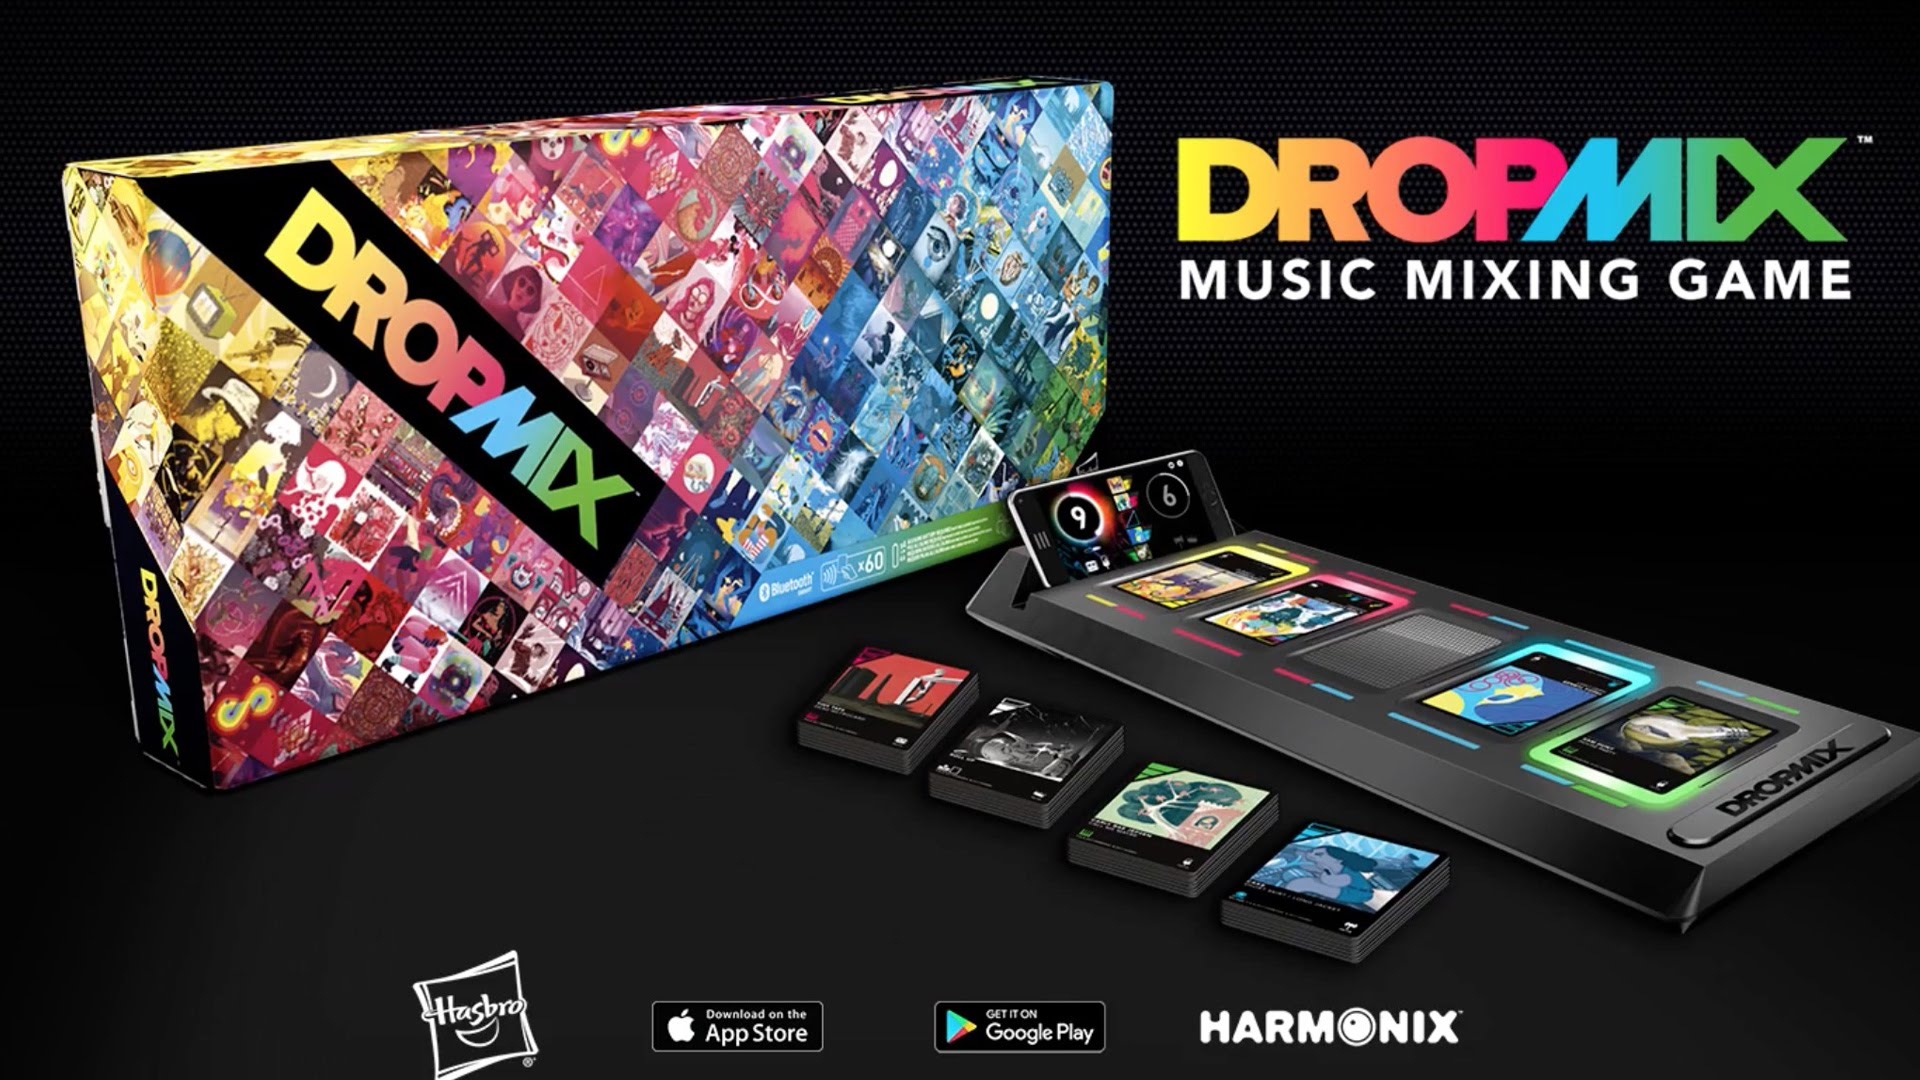
\includegraphics[width=0.7\linewidth]{figure/Analysis/dropmix}
	\caption{Shows the Drop mix package}
	\label{fig:dropmix}
\end{figure}


\subsection{Dance Dance Revolution}
Dance Dance Revolution(DDR) is a physical interactive dance platform created by the Japanese company Konami, and can be seen in \autoref{fig:dancedance}. Players will stand on the platform and step on the colored arrows on the stand of the platform, corresponding to the arrows that will be shown on the screen. DDR's design makes use constructive competition and cooperative learning.

From the workshop it was found that many of the children wanted movement. DDR incorporates movement and physicality, which can be connected to learning as mentioned in \autoref{interaction}.
\todo{and summarize section}
\begin{figure}[H]
	\centering
	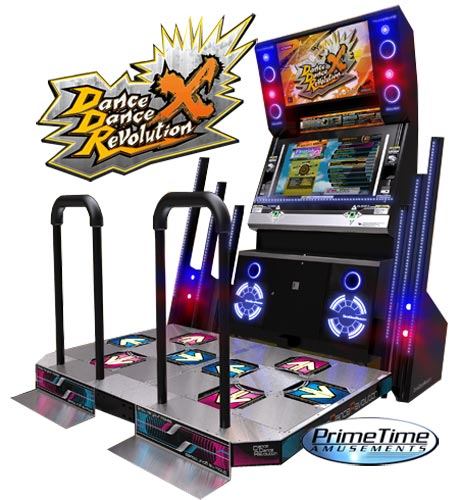
\includegraphics[width=0.7\linewidth]{figure/Analysis/dancedance}
	\caption{shows the arcade version of the DDR controller}
	\label{fig:dancedance}
\end{figure}

\subsection{Just dance}
Just dance is a dance video game developed by Ubisoft Milan and Ubisoft Paris. The game was released mainly for usage on the Nintendi Wii. The whole idea about the game is that each user must mimic the motions of an onscreen dancer’s choreography. For each movement the user will get more points, and the more correct the movements are the more points the user will receive. A screenshot of the game can be seen in \autoref{fig:justDance}.

As the workshop concludes it is very important for the children to be able to move, and Just Dance adds the capability of moving freely around the room as long as the person is still within the range of the sensor.

\begin{figure}[H]
	\centering
	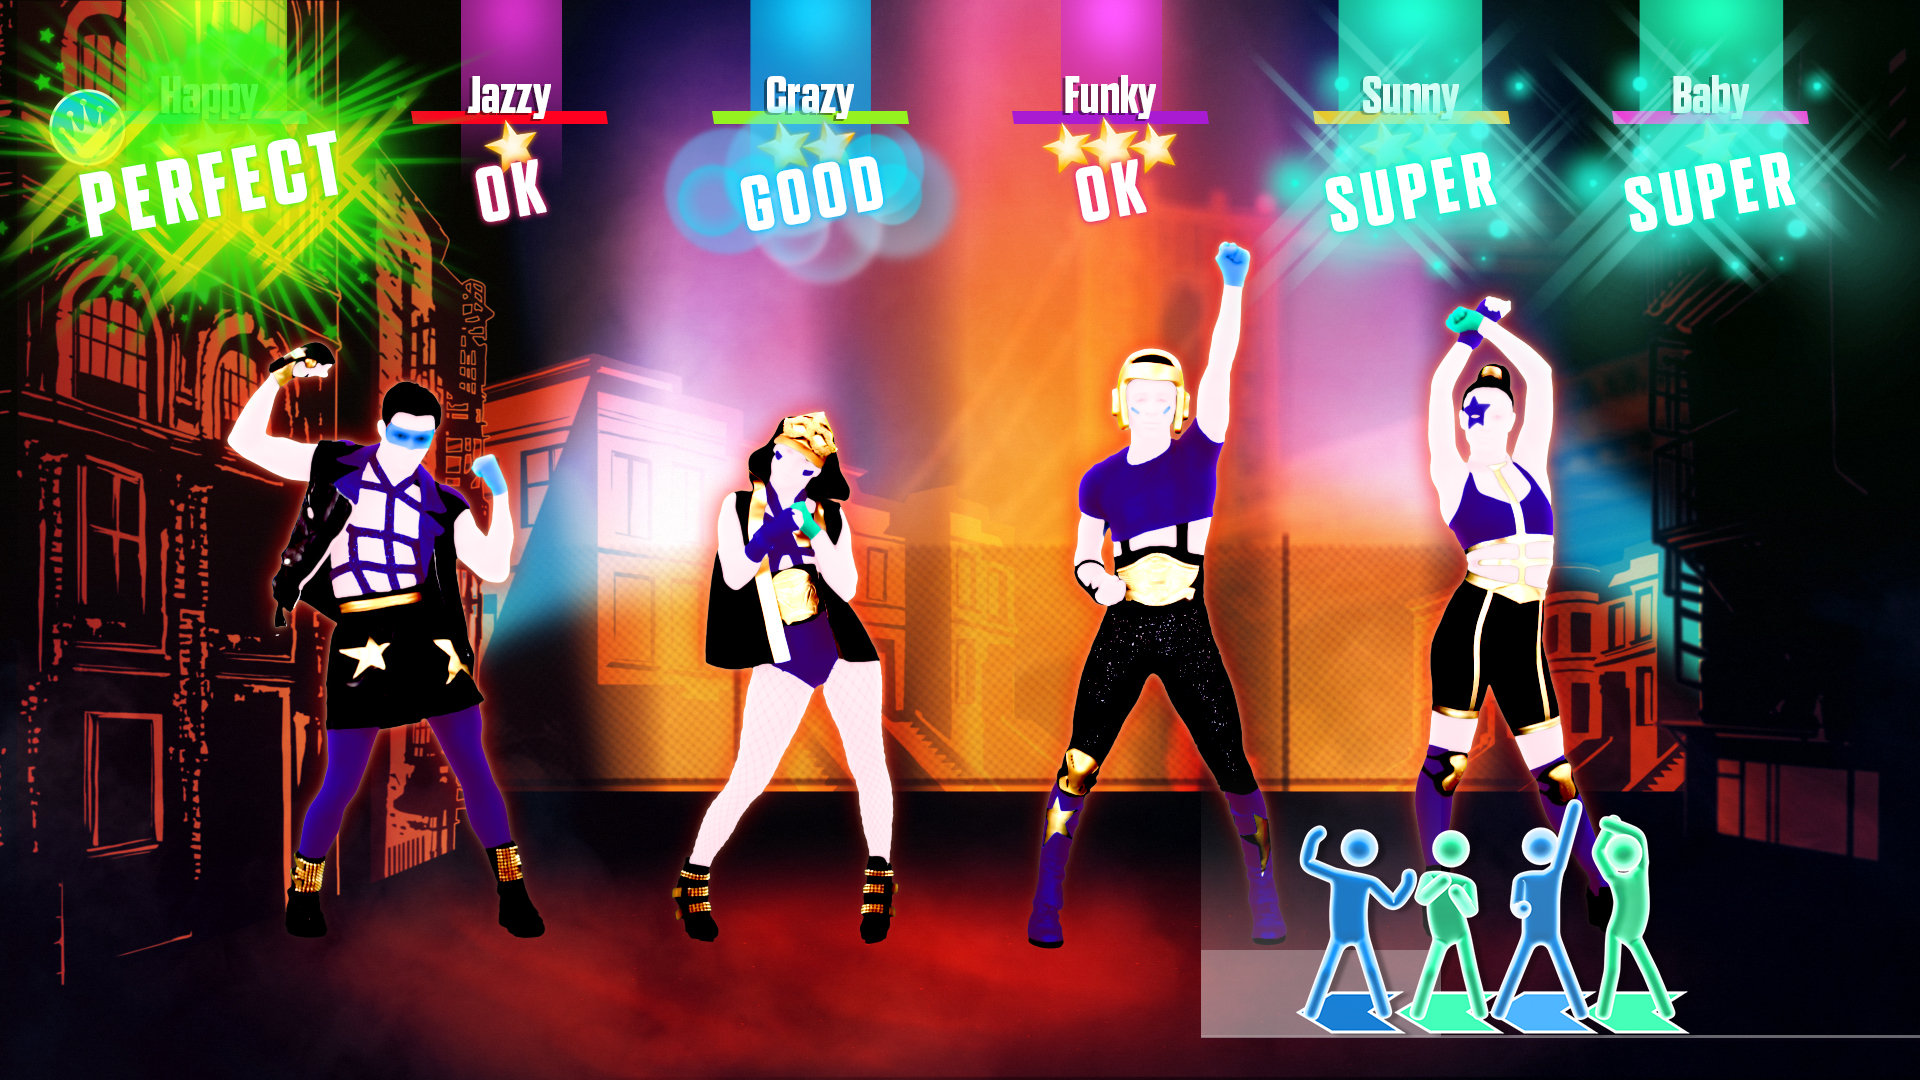
\includegraphics[width=0.7\linewidth]{figure/Analysis/justdance}
	\caption{Shows the games interface}
	\label{fig:justDance}
\end{figure}

\subsection{Gridi}
Gridi is a physical board, which functions as a sequencer. Gridi has a 16x16 grid of different holes, which can play sound, and can be seen in figure \autoref{fig:Gridi}. When a ball is placed in one of these holes it will be enabled. Gridi iterates over each line and plays sound according to the placement of the balls. Gridi is a cooperative tool, since multiple users can use it simultaneously.

\begin{figure}[H]
	\centering
	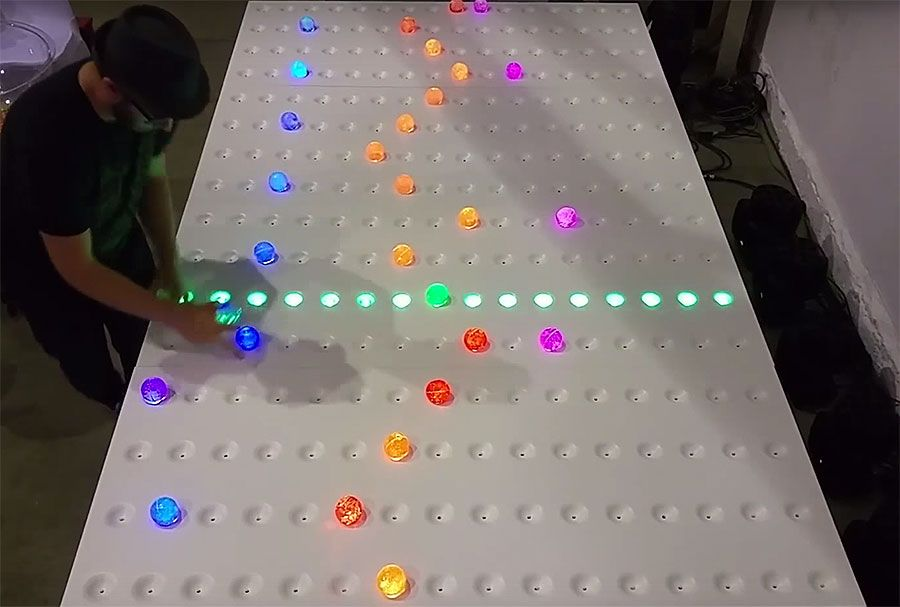
\includegraphics[width=0.7\linewidth]{figure/Analysis/gridi}
	\caption{Shows the Gridi interface, and the sequencer looping through the table.}
	\label{fig:Gridi}
\end{figure}

\subsection*{Sub Conclusion}
The state of the art will help shape the design requirements. They will work as inspiration for specific design features and implementations. The current tools that teach music, vary a lot in the aspects they focus on, some focus on playing, some on movement, some are based on a hardware product, and some on software. All of these individual products could be utilized as inspiration in the design phase.

\section{Analysis summary}
The initial analysis investigated and found that there is a consensus between learning music and developing other aspects of life. This led to further investigation in learning in general, where it was found that there are two main concepts of learning; passive and active learning. Active learning displayed a lot of positive results through interactions and emotions, which lead to research in these areas. In motivation theory, the concept of Cognitive Evaluation Theory(CET) was discovered. The CET argues that humans have more motivation working in groups, as they get social-contextual events, praise or other rewards. Furthermore, collaborative learning enhances various aspects of learning. Specifically, when it comes to music, collaborative work strengthens the understanding of concepts and enhances critical thinking.\\

In order to establish a target group, the study plan was investigated, and a music teacher was interviewed, to highlight issues with current musical education. It was found that there was a need for physical tools that elementary school students could use in collaboration with each other. A workshop was held with students at Skt. Annæ Skole, where several design and functionality ideas were presented. The feedback provided, gave an understanding of what kind of tool the students themselves wanted, on top of what the teacher had already provided as feedback. Therefore, the solution would be a physical tool, that the students could use in collaboration with each other in an elementary school setting.\\

Further investigation lead to a better understanding of the concepts of group work, group roles, and the three different collaborative learning methods; cooperative learning, constructive competition and peer learning.\\


\section{Final Problem Statement}\label{sec:FPS}
	How can a physical interface facilitate collaboration in small groups for elementary school children, aged 8-12 years in a musical education context?

	
\section{Design Requirements}\label{sec:DRequirements}

The following requirements, based on the analysis, are the physical framework that the design should strive to fulfill.
	\subsection*{Requirements}
		\begin{itemize}
			\item[-] It must accommodate at least 2 children.\\
			\item[-] It must accommodate max 6 children.\\
			\item[-] Must facilitate collaboration within at least one of the three musical areas of competence.\\
			\item[-] Must be designed for Children aged 8-12.\\
			\item[-] It should strive to not induce  negative emotions.\\
			\item[-] It should strive to induce positive emotions.\\
			\item[-] It must output sound.	\\	
			\item[-] It must be interactable.\\
			\item[-] It must have a physical interface.\\
		\end{itemize}
	
















		